\documentclass[11pt,a4paper]{article}

\usepackage[utf8]{inputenc}
\usepackage[T1]{fontenc}
\usepackage[margin=2.5cm]{geometry}
\usepackage{amsmath,amssymb,amsthm}
\usepackage{float}
\usepackage{algorithm}
\usepackage[noend]{algpseudocode}
\usepackage{booktabs}
\usepackage{tikz}
\usetikzlibrary{positioning,decorations.pathreplacing}
\usepackage[hidelinks]{hyperref}

\newtheorem{proposition}{Proposition}
\theoremstyle{remark}
\newtheorem*{remark}{Remark}

\algnewcommand\algorithmicto{\textbf{to}}
\algnewcommand{\Continue}{\State \textbf{continue}}
\algnewcommand{\Error}[1]{\State \textbf{error} ``#1''}
\algrenewcommand\algorithmicrequire{\textbf{Input:}}
\algrenewcommand\algorithmicensure{\textbf{Output:}}

\newcommand{\dist}{\mathrm{dist}}
\newcommand{\seen}{\mathrm{seen}}
\newcommand{\owner}{\mathrm{owner}}
\newcommand{\paths}{\mathrm{paths}}
\newcommand{\cell}{\mathrm{cell}}

\title{Weighted graph Voronoi cells\\[2pt]
\large Algorithms of \texttt{voronoi.py}}
\author{Network Expansion Planning -- EDF project}
\date{\today}

\begin{document}
\maketitle

\begin{abstract}
The first step of the Voronoi + Steiner heuristic splits the nodes of the
network between the sources (substations). Each node is assigned to the source
that reaches it at the smallest \emph{scaled} cost, where every edge length on
a path starting at source $s$ is divided by a weight $w_s$ of that source.
This document gives the algorithms of \texttt{voronoi.py} in pseudocode: the
weighted multi-source Dijkstra, the construction of the cells, the splitting of
the edges lying between two cells, and the shortest-path trees. It also states
the properties these algorithms guarantee, then works through a small example.
\end{abstract}

\section{Setting and notation}

\begin{itemize}
  \item $G=(V,E)$ is an undirected graph. Each edge $(u,v)$ has a length
        $\ell(u,v)\ge 0$ (attribute \texttt{weight}, in km). Each node has a
        \texttt{label}, a position $\mathrm{pos}(v)\in\mathbb{R}^2$ and a power
        \texttt{conso\_ete}.
  \item $S=\{v\in V : \mathrm{label}(v)=\texttt{Source}\}$ is the set of sources.
  \item Each source $s$ has a weight $w_s>0$ (Algorithm~\ref{alg:weight}). Every
        edge on a path that starts at $s$ costs $\ell(u,v)/w_s$. A larger
        weight makes $s$ look closer, so its cell grows.
  \item $N(v)$ is the set of neighbours of $v$ in $G$.
\end{itemize}

The algorithms return, for each node $v$, its scaled distance $\dist(v)$, its
source $\sigma(v)\in S$ and a path $\paths(v)$ from $\sigma(v)$ to $v$. The cell
of a source $s$ is $C_s=\{v : \sigma(v)=s\}$.

Table~\ref{tab:map} links each algorithm to its function in the code.

\begin{table}[H]
\centering
\begin{tabular}{@{}lll@{}}
\toprule
Algorithm & Name & Python function \\
\midrule
\ref{alg:weight}   & \textsc{SourceWeight}          & \texttt{source\_weight} \\
\ref{alg:dijkstra} & \textsc{DijkstraMultisourceSB} & \texttt{\_dijkstra\_multisource\_SB}, \\
                   &                                & \texttt{multi\_source\_dijkstra\_SB} (wrapper) \\
\ref{alg:cells}    & \textsc{VoronoiCellsSB}        & \texttt{voronoi\_cells\_SB} \\
                   & \textsc{CellsFromPaths}        & \texttt{cells\_from\_paths} \\
\ref{alg:split}    & \textsc{VoronoiCellsEdges}     & \texttt{voronoi\_cells\_edges} \\
\ref{alg:trees}    & \textsc{EdgesOnShortestPaths}  & \texttt{edges\_on\_shortest\_paths} \\
\ref{alg:main}     & \textsc{ComputeVoronoiCells}   & \texttt{compute\_voronoi\_cells} \\
\bottomrule
\end{tabular}
\caption{Algorithms of this document and the corresponding functions of \texttt{voronoi.py}.}
\label{tab:map}
\end{table}

\section{Source weights}

Four weightings are available. Three are fixed: \texttt{none}, \texttt{capacity}
and \texttt{sqrt}. The fourth is a dictionary of free weights, which the
variable-distance method (\texttt{voronoi\_variable\_distance.py}) adjusts
iteratively.

\begin{algorithm}[H]
\caption{Weight of a source}\label{alg:weight}
\begin{algorithmic}[1]
\Function{SourceWeight}{$G, s, \mathit{weighting}$}
  \If{$\mathit{weighting}$ is a dictionary}
    \State \Return $\mathit{weighting}[s]$ \Comment{free weights}
  \EndIf
  \If{$\mathit{weighting}=\texttt{none}$} \State \Return $1$ \EndIf
  \State $c \gets \texttt{conso\_ete}(s)$ \Comment{capacity of the source, must be $>0$}
  \If{$\mathit{weighting}=\texttt{capacity}$} \State \Return $c$ \EndIf
  \If{$\mathit{weighting}=\texttt{sqrt}$} \State \Return $\sqrt{c}$ \EndIf
  \Error{unknown weighting}
\EndFunction
\end{algorithmic}
\end{algorithm}

\section{Weighted multi-source Dijkstra}

This is the core of the method. It is the multi-source Dijkstra of
\texttt{networkx} with one change: when a settled node $v$ relaxes its
neighbours, the cost of each edge is divided by the weight of $v$'s source, and
an improved neighbour inherits that source.

\begin{algorithm}[H]
\caption{Multi-source Dijkstra with costs scaled by the source weight}\label{alg:dijkstra}
\begin{algorithmic}[1]
\Require graph $G$, non-empty set of sources $S\subseteq V$, weighting
\Ensure $\dist$: scaled distance of each reached node; $\paths$: path from its source
\Function{DijkstraMultisourceSB}{$G, S, \mathit{weighting}$}
  \State $\dist \gets \emptyset$;\quad $\paths\gets\emptyset$
  \State $\seen \gets \emptyset$ \Comment{best tentative distances}
  \State $\owner \gets \emptyset$ \Comment{tentative source of each node}
  \State $H \gets$ empty min-heap of triples $(d, c, v)$;\quad $c \gets 0$
         \Comment{counter $c$ breaks ties}
  \ForAll{$s \in S$}
    \State $\seen(s)\gets 0$;\quad $\owner(s)\gets s$;\quad $\paths(s)\gets [s]$
    \State push $(0, c, s)$ on $H$;\quad $c\gets c+1$
  \EndFor
  \While{$H \neq \emptyset$}
    \State $(d, \cdot, v) \gets$ pop the minimum of $H$
    \If{$v \in \dist$} \Continue \Comment{stale entry: $v$ already settled}
    \EndIf
    \State $\dist(v) \gets d$ \Comment{$v$ is settled: $d$ and $\owner(v)$ are final}
    \State $s \gets \owner(v)$;\quad $w_s \gets$ \Call{SourceWeight}{$G, s, \mathit{weighting}$}
    \ForAll{$u \in N(v)$}
      \State $\delta \gets \dist(v) + \ell(v,u)/w_s$ \Comment{cost scaled by the weight of $v$'s source}
      \If{$u \in \dist$}
        \If{$\delta < \dist(u)$} \Error{contradictory paths: negative weights?} \EndIf
      \ElsIf{$u \notin \seen$ \textbf{or} $\delta < \seen(u)$} \Comment{strict: ties keep the first owner}
        \State $\seen(u) \gets \delta$;\quad $\owner(u) \gets s$
        \State $\paths(u) \gets \paths(v) + [u]$
        \State push $(\delta, c, u)$ on $H$;\quad $c\gets c+1$
      \EndIf
    \EndFor
  \EndWhile
  \State \Return $\dist, \paths$
\EndFunction
\end{algorithmic}
\end{algorithm}

The wrapper \texttt{multi\_source\_dijkstra\_SB} first checks that $S\neq\emptyset$
and $S\subseteq V$, then calls Algorithm~\ref{alg:dijkstra}.

\paragraph{Properties.} Write $\sigma(v)=\paths(v)[0]$ for the source of a
settled node $v$, and $C_s=\{v:\sigma(v)=s\}$.

\begin{proposition}[Settling order]\label{prop:order}
Nodes are settled in nondecreasing order of $\dist$. If all lengths are
nonnegative, the error on the contradictory-paths line is never raised.
\end{proposition}
\begin{proof}
Every pushed key is $\dist(v)+\ell(v,u)/w_s\ge\dist(v)$, and $v$ is the current
minimum of the heap, so keys pushed later are never below those already popped.
If $u$ was settled before $v$, then $\dist(u)\le\dist(v)\le\delta$.
\end{proof}

\begin{proposition}[Connected cells]\label{prop:connected}
For every settled $v$, every node of $\paths(v)$ lies in $C_{\sigma(v)}$. So
each cell $C_s$ is connected and contains $s$, and the union of the paths of a
cell is a tree rooted at $s$.
\end{proposition}
\begin{proof}
$\paths(u)$ is set to $\paths(v)+[u]$ at the same moment as $\owner(u)\gets\owner(v)$,
and $\owner(v)$ is already final. By induction on the settling order, every
prefix of $\paths(u)$ is the path of a node of the same cell. The paths are
nested prefixes, so their union is a tree.
\end{proof}

\begin{proposition}[What $\dist$ is]\label{prop:dist}
For every settled $v$,
\[
\dist(v)=\frac{d_{G[C_{\sigma(v)}]}\bigl(\sigma(v),v\bigr)}{w_{\sigma(v)}},
\]
where $d_{G[C]}$ is the shortest-path distance in the subgraph induced by $C$.
Moreover, for every source $s'$ and every path $P$ from $s'$ to $v$ whose
nodes, $v$ excepted, all lie in $C_{s'}$, we have $\dist(v)\le \ell(P)/w_{s'}$.
\end{proposition}
\begin{proof}[Sketch]
Inside a cell all edges are scaled by the same factor $1/w_s$, so the usual
Dijkstra argument applies to $G[C_s]$. For the second claim, each node $x$ of
$P$ is settled with owner $s'$ and relaxes its successor on $P$ with cost
$\dist(x)+\ell/w_{s'}$. By induction, $\dist(v)\le\ell(P)/w_{s'}$.
\end{proof}

\begin{remark}
This differs from the classical multiplicatively weighted Voronoi diagram,
where $v$ would go to $\arg\min_s d_G(s,v)/w_s$. Here a source cannot extend a
path through a node another source has already settled. As a result the cells
are always connected (Proposition~\ref{prop:connected}), which the Steiner step
needs. In the classical diagram, the cell of a strong source can surround a
weak one or be cut into several pieces.
\end{remark}

\paragraph{Complexity.} Each edge is relaxed at most twice and each relaxation
pushes at most one heap entry. With a binary heap, the running time is
$O\bigl((|V|+|E|)\log|V|\bigr)$, like standard Dijkstra. The paths
$\paths(u)=\paths(v)+[u]$ are copied explicitly, which costs $O(|V|\cdot h)$
memory, where $h$ is the largest number of nodes on a path.

\section{Voronoi cells}

\begin{algorithm}[H]
\caption{Voronoi cells from the shortest paths}\label{alg:cells}
\begin{algorithmic}[1]
\Function{VoronoiCellsSB}{$G, S, \mathit{weighting}$}
  \State $\dist, \paths \gets$ \Call{DijkstraMultisourceSB}{$G, S, \mathit{weighting}$}
  \State $\mathit{cells} \gets$ \Call{CellsFromPaths}{$G, \paths$}
  \State \Return $\dist, \mathit{cells}, \paths$
\EndFunction
\Statex
\Function{CellsFromPaths}{$G, \paths$}
  \State $\mathit{cells} \gets \emptyset$ \Comment{source $\mapsto$ set of nodes}
  \ForAll{$(v, p) \in \paths$}
    \State $\mathit{cells}[p[0]] \gets \mathit{cells}[p[0]] \cup \{v\}$
           \Comment{first node of the path is the source}
  \EndFor
  \State $R \gets V \setminus \mathrm{keys}(\paths)$ \Comment{nodes reached by no source}
  \If{$R\neq\emptyset$} \State $\mathit{cells}[\texttt{unreachable}] \gets R$ \EndIf
  \State \Return $\mathit{cells}$
\EndFunction
\end{algorithmic}
\end{algorithm}

\section{Splitting the edges between two cells}

An edge $(u,v)$ of length $\ell$ whose ends lie in two different cells is cut
at the point $q$ that is equidistant from both sources in the scaled metric.
Write $w_u=w_{\sigma(u)}$ and $w_v=w_{\sigma(v)}$, and place $q$ at distance
$t\ell$ from $u$, with $t\in[0,1]$. The condition
\[
\dist(u) + \frac{t\,\ell}{w_u} \;=\; \dist(v) + \frac{(1-t)\,\ell}{w_v}
\]
gives
\begin{equation}\label{eq:t}
t \;=\; \frac{\bigl(\dist(v)-\dist(u)\bigr)\,\dfrac{w_u w_v}{\ell} + w_u}{w_u+w_v}
\qquad(\ell\neq 0),
\end{equation}
and the code takes $t=1$ when $\ell=0$.

\begin{proposition}\label{prop:t}
If $\dist$ comes from Algorithm~\ref{alg:dijkstra} with the same weighting,
then $t\in[0,1]$ for every boundary edge.
\end{proposition}
\begin{proof}
When $v$ was settled, it relaxed $u$ with cost $\dist(v)+\ell/w_v$. If $u$ was
still unsettled, $u$'s final distance is at most that cost. If $u$ was already
settled, $\dist(u)\le\dist(v)$ by Proposition~\ref{prop:order}. Either way,
$\dist(u)-\dist(v)\le \ell/w_v$, which is equivalent to $t\ge 0$ in
\eqref{eq:t}. Exchanging the roles of $u$ and $v$ gives
$\dist(v)-\dist(u)\le\ell/w_u$, which is equivalent to $t\le 1$.
\end{proof}

The code still checks $t\in[-10^{-9},1+10^{-9}]$ and then clamps $t$ to
$[0,1]$. A larger deviation means that the cells and the distances were
computed with different weightings.

\begin{algorithm}[H]
\caption{Assign the edges to the cells and split the boundary edges ($G$ is modified)}\label{alg:split}
\begin{algorithmic}[1]
\Require cells without the key \texttt{unreachable}; $\dist$ from the same weighting; $V=\{0,\dots,|V|-1\}$
\Ensure edges of each cell, the split nodes, the distance of each split node to both sources
\Function{VoronoiCellsEdges}{$G, \mathit{cells}, \dist, \mathit{weighting}$}
  \If{$\texttt{unreachable}\in\mathit{cells}$} \Error{some nodes are reachable from no source} \EndIf
  \State $E_k \gets [\,]$ for each cell $k$;\quad $E_{\texttt{split}}\gets[\,]$
  \State $\cell(n) \gets k$ for each cell $k$ and each $n \in \mathit{cells}[k]$
  \State $\mathit{next} \gets |V|$ \Comment{ids of the new nodes}
  \State $\mathit{toAdd} \gets [\,]$;\quad $D \gets \emptyset$
  \ForAll{$(u,v)\in E$ with length $\ell$}
    \If{$\cell(u)=\cell(v)$}
      \State append $(u,v)$ to $E_{\cell(u)}$ \Comment{inner edge}
      \Continue
    \EndIf
    \State $w_u \gets$ \Call{SourceWeight}{$G,\cell(u),\mathit{weighting}$}
    \State $w_v \gets$ \Call{SourceWeight}{$G,\cell(v),\mathit{weighting}$}
    \If{$\ell\neq 0$}
      \State $t \gets \Bigl(\bigl(\dist(v)-\dist(u)\bigr)\,w_u w_v/\ell + w_u\Bigr)\big/(w_u+w_v)$
             \Comment{equation~\eqref{eq:t}}
    \Else
      \State $t\gets 1$
    \EndIf
    \If{$t<-10^{-9}$ \textbf{or} $t>1+10^{-9}$} \Error{split point outside the edge} \EndIf
    \State $t\gets \min(\max(t,0),1)$
    \State $q \gets \mathit{next}$;\quad $\mathit{next}\gets\mathit{next}+1$
    \State $\mathrm{pos}_q \gets \mathrm{pos}(u) + t\,\bigl(\mathrm{pos}(v)-\mathrm{pos}(u)\bigr)$
           \Comment{linear interpolation}
    \State append $(q,\mathrm{pos}_q,u,v,\,t\ell,\,(1-t)\ell)$ to $\mathit{toAdd}$
    \State append $(u,q)$ to $E_{\cell(u)}$;\quad append $(v,q)$ to $E_{\cell(v)}$
           \Comment{one half-edge per cell}
    \State append $(u,v)$ to $E_{\texttt{split}}$
    \State $D(q) \gets \bigl\{\cell(u): \dist(u)+t\ell/w_u,\;\; \cell(v): \dist(v)+(1-t)\ell/w_v\bigr\}$
           \Comment{equal values}
  \EndFor
  \ForAll{$(q,\mathrm{pos}_q,u,v,l_1,l_2)\in\mathit{toAdd}$}
    \Comment{after the loop over $E$}
    \State add node $q$ to $G$ with label \texttt{dummy} and position $\mathrm{pos}_q$
    \State add edges $(u,q)$ of length $l_1$ and $(v,q)$ of length $l_2$, label \texttt{dummy}
    \Comment{$(u,v)$ is kept}
  \EndFor
  \State \Return $(E_k)_k \cup \{E_{\texttt{split}}\},\ \mathit{toAdd},\ D$
\EndFunction
\end{algorithmic}
\end{algorithm}

\section{Shortest-path trees of the cells}

The edges used by the shortest paths of a cell form a tree rooted at its source
(Proposition~\ref{prop:connected}). This tree is the ``Voronoi-only'' network,
before the Steiner step.

\begin{algorithm}[H]
\caption{Edges on the shortest paths of each cell}\label{alg:trees}
\begin{algorithmic}[1]
\Function{EdgesOnShortestPaths}{$\mathit{cells}, \paths$}
  \ForAll{cell $k$}
    \State $U_k \gets \emptyset$
    \ForAll{$n\in\mathit{cells}[k]$}
      \State $p \gets \paths(n)$
      \For{$i \gets 0$ \algorithmicto\ $|p|-2$}
        \State $U_k \gets U_k \cup \bigl\{(\min(p_i,p_{i+1}),\,\max(p_i,p_{i+1}))\bigr\}$
      \EndFor
    \EndFor
  \EndFor
  \State \Return $\{k : \mathrm{sorted}(U_k)\}$
\EndFunction
\end{algorithmic}
\end{algorithm}

\section{Entry point}

Algorithm~\ref{alg:main} runs the whole pipeline and stores the results in the
\texttt{GraphData} object. The original graph is not modified. The split
edges are added to a copy, $G_{\text{split}}$, which is used only for plotting.
The Steiner step that follows runs on the original $G$, using the node cells.

\begin{algorithm}[H]
\caption{Voronoi cells of the sources of a network}\label{alg:main}
\begin{algorithmic}[1]
\Procedure{ComputeVoronoiCells}{$\mathit{graph}, \mathit{weighting}$}
  \State $G \gets \mathit{graph}.G$;\quad $S\gets\{n\in V : \mathrm{label}(n)=\texttt{Source}\}$
  \State $\mathit{graph}.\dist,\ \mathit{graph}.\mathit{cells},\ \mathit{graph}.\paths \gets$
         \Call{VoronoiCellsSB}{$G, S, \mathit{weighting}$}
  \State $\mathit{graph}.\mathit{usedEdges} \gets$
         \Call{EdgesOnShortestPaths}{$\mathit{graph}.\mathit{cells}, \mathit{graph}.\paths$}
  \State $G_{\text{split}} \gets$ copy of $G$
  \State $\mathit{cells}\gets\mathit{graph}.\mathit{cells}$;\quad $\dist\gets\mathit{graph}.\dist$
  \State $\mathit{graph}.\mathit{edgeCells},\ \mathit{toAdd},\ \cdot \gets$
         \Call{VoronoiCellsEdges}{$G_{\text{split}}, \mathit{cells}, \dist, \mathit{weighting}$}
  \State $\mathit{graph}.G_{\text{split}} \gets G_{\text{split}}$
  \ForAll{$(q,\mathrm{pos}_q,u,v,\cdot,\cdot)\in\mathit{toAdd}$} \Comment{plotting only}
    \State add point $q$ and segments $u\to q$, $v\to q$ to copies of the node and edge tables
  \EndFor
\EndProcedure
\end{algorithmic}
\end{algorithm}

\section{Worked example}

Consider the path graph of Figure~\ref{fig:example}, with capacity weighting
$w_{S_1}=3$, $w_{S_2}=1$ and all edge lengths equal to $3$.

\begin{figure}[H]
\centering
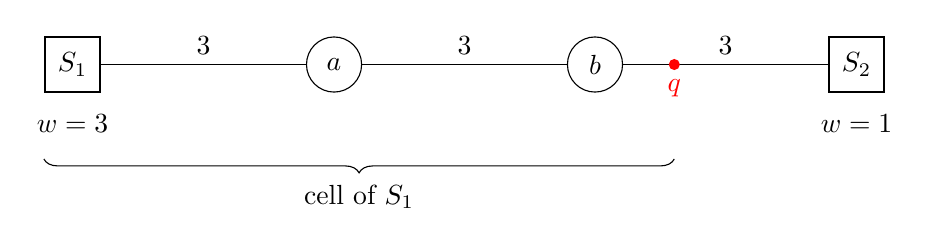
\begin{tikzpicture}[node distance=2.6cm,
    src/.style={rectangle,draw,thick,minimum size=7mm},
    load/.style={circle,draw,minimum size=7mm}]
  \node[src]  (s1) {$S_1$};
  \node[load] (a)  [right=of s1] {$a$};
  \node[load] (b)  [right=of a]  {$b$};
  \node[src]  (s2) [right=of b]  {$S_2$};
  \draw (s1) -- node[above]{3} (a);
  \draw (a)  -- node[above]{3} (b);
  \draw (b)  -- coordinate[pos=0.25] (q) node[above]{3} (s2);
  \fill[red] (q) circle (2pt) node[below=2pt,red] {$q$};
  \node[below=0.15cm of s1] {$w=3$};
  \node[below=0.15cm of s2] {$w=1$};
  \draw[decorate,decoration={brace,mirror,amplitude=5pt}]
       ([yshift=-1.2cm]s1.west) -- ([yshift=-1.2cm]q) node[midway,below=6pt]{cell of $S_1$};
\end{tikzpicture}
\caption{The source $S_1$ is three times stronger than $S_2$: its cell takes
$b$, and the boundary point $q$ is three times closer to $S_2$ than to $S_1$
($2.25$ km against $6.75$ km).}
\label{fig:example}
\end{figure}

Table~\ref{tab:run} traces Algorithm~\ref{alg:dijkstra}.

\begin{table}[H]
\centering
\begin{tabular}{@{}clll@{}}
\toprule
Step & Popped (owner) & Relaxations & Heap afterwards \\
\midrule
1 & $S_1$ $(0)$         & $a$: $0+3/3=1$, owner $S_1$                    & $(0,S_2), (1,a)$ \\
2 & $S_2$ $(0)$         & $b$: $0+3/1=3$, owner $S_2$                    & $(1,a), (3,b)$ \\
3 & $a$ $(1, S_1)$      & $b$: $1+3/3=2<3$, $b$ moves to $S_1$            & $(2,b), (3,b)$ \\
4 & $b$ $(2, S_1)$      & $S_2$ already settled, $2+1\ge 0$, nothing to do & $(3,b)$ \\
5 & $b$ $(3)$           & stale entry, skipped                           & empty \\
\bottomrule
\end{tabular}
\caption{Run of the weighted Dijkstra on the example.}
\label{tab:run}
\end{table}

The result is $C_{S_1}=\{S_1,a,b\}$ and $C_{S_2}=\{S_2\}$: although $b$ is
closer to $S_2$ in plain kilometres, the stronger source takes it. The only
boundary edge is $(b,S_2)$, with $\ell=3$, $\dist(b)=2$, $\dist(S_2)=0$,
$w_u=3$ and $w_v=1$. Equation~\eqref{eq:t} gives
\[
t=\frac{(0-2)\cdot 3\cdot 1/3+3}{3+1}=\frac14,
\]
so $q$ is $0.75$ km from $b$ and $2.25$ km from $S_2$. As a check, the scaled
distance to $q$ is $2+0.75/3=2.25$ from the $S_1$ side and $0+2.25/1=2.25$
from the $S_2$ side.

\end{document}
